\documentclass[a4paper]{article}

\usepackage[english]{babel}
\usepackage[utf8]{inputenc}
\usepackage{amsmath}
\usepackage{graphicx}
\usepackage{wrapfig}
\usepackage{subfigure}
\usepackage[colorinlistoftodos]{todonotes}

\title{Computing Water Volume in a Tilted Cup}


\begin{document}
\date{}
\maketitle

\section{Introduction}

One day when drinking water, I noticed that there is a non-symmetry between the geometric space up and below water surface inside a tilted cup. A circular cylinder is in a nice shape. A water cup, with top surface enlarged compared to a standard cylinder, is almost as nice but not quite. I did some computation for the volume of the remaining water in a tilted cup, as shown in figure \ref{fig:1}.

\begin{figure}[h]
\centering
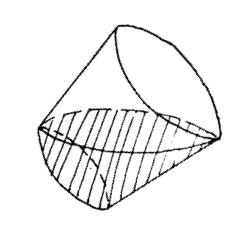
\includegraphics[width=0.25\textwidth]{fig/1.png}
\caption{\label{fig:1}Water surface cuts the top rim of a tilted cup.}
\end{figure}

\section{Steps}

\subsection{First Inspection}

\begin{wrapfigure}{h}{0.25\textwidth}
\centering
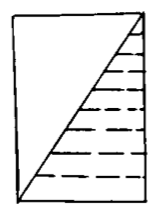
\includegraphics[width=0.2\textwidth]{fig/2.png}
\caption{\label{fig:2}Side view of the cylinder cup.}
\end{wrapfigure}

An intuition is that simplified problem with a cylinder setting gives hint on the more generalized and realistic case. Say the cup has top and bottom to be circular with same radii $r$ as figure \ref{fig:2}. 



Horizontally slice the cylinder into $n$ pieces and each piece has a small thickness of $l/n$. For each horizontal slice which has height $h$, which is the distance from the bottom, water surface and the slice intersects at a chord with half length $x$. See figure \ref{fig:3}, \ref{fig:4}.\\


\begin{figure}[t]
\centering
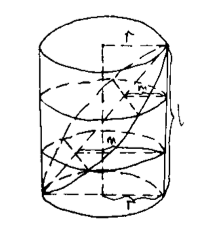
\includegraphics[width=0.25\textwidth]{fig/3.png}
\caption{\label{fig:3}3-D view of the cylinder cup.}
\end{figure}

\begin{figure}[h]
\centering
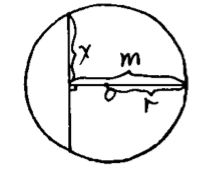
\includegraphics[width=0.2\textwidth]{fig/4.png}
\caption{\label{fig:4}One slice.}
\end{figure}


By property of similar triangles, 
\[\frac{l - h}{l} = \frac{m}{2r}\]
This gives
\[x = \sqrt{r^2 - (m-r)^2} = \frac{2r}{l}\sqrt{h(l-h)}\]
Notice the symmetry of $h$ and $l-h$, corresponding to two slices with equal distance from the center of the cylinder. The 2-D area where a certain slice is emerged in water is part of the circular face with radii $r$. For two slices with height $h$ and $l-h$, two areas complete the circular face, thus with and area of $\pi r^2$ in total and a volume of $\pi r^2 \frac{l}{n}$. \\
The total volume of water follows as
\[V = \frac{n}{2} \dot \pi r^2 \frac{l}{n} = \frac{1}{2}\pi r^2 l\]
Volume of water is exactly half volume of the cylinder.





\subsection{Second Construction}


\begin{figure}[b]
\centering
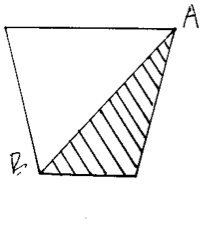
\includegraphics[width=0.2\textwidth]{fig/5.png}
\caption{\label{fig:5}Slice in parallel to water surface.}
\end{figure}
\begin{figure}[t]
\centering
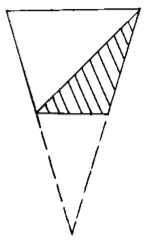
\includegraphics[width=0.2\textwidth]{fig/6.png}
\caption{\label{fig:6}Cup extended to cone.}
\end{figure}


When the cup is not perfect cylinder, horizontal slices do not help much because radii of each slice is no longer the same. However, the idea of slicing still sounds intriguing. What about chopping the cup into slices parallel to the water surface, rather than the top or bottom surface? See figure \ref{fig:5}.\\
To make it even nicer, extend the cup into a cone so that each slice resides a complete ellipse, as in figure \ref{fig:6}.\\



\subsection{Computation}

\begin{figure}[b]
\centering
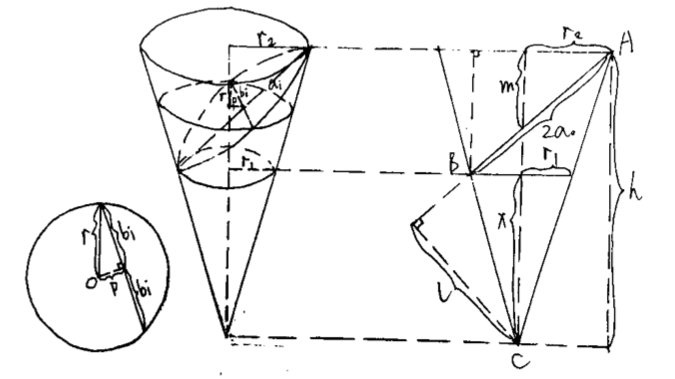
\includegraphics[width=0.7\textwidth]{fig/78.png}
\caption{\label{fig:78}Left hand side is the horizontal slice going through the minor semi-axis.}
\end{figure}

Let $r_1, r_2$ be the radii of top and bottom surface, where $r_1 > r_2$ based on life experience. Denote the height of the extended cone as $h$, the vertical distance from water surface to the center of top surface as $m$, and the vertical distance from cone apex to the center of bottom surface as $x$.\\
Now chop the cone into $n$ slices parallel to water surface. Consider the $i$-th slice, an eclipse with semi-axes of length $a_i, b_i$ where $a_i > b_i$. Let $h_i$ be the vertical distance from the cone apex to the slice.\\
By property of similar triangles in figure \ref{fig:78},
\[\frac{h}{r_2} = \frac{x}{r_1}\]
\[\frac{m}{h-x} = \frac{r_1}{r_2}\]
For $i$-th slice: 
\[h_i = (h-m) - \frac{h-m}{n}\dot i\]
\[2 a_i = \frac{h_i}{h - m} \dot 2a_0\]
\[a_i = \frac{n-i}{n} a_0\]



\begin{wrapfigure}{r}{0.25\textwidth}
\centering
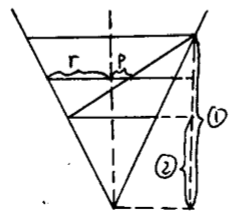
\includegraphics[width=0.2\textwidth]{fig/9.png}
\caption{\label{fig:9}Side view of $i$-th slice.}
\end{wrapfigure}

To compute $b_i$, let $p$, $\alpha$, $\beta$ as the measures illustrated in \ref{fig: 9}.
\[\alpha = h_i + \frac{h-x}{2a_0}2 a_i \frac{m}{h-x} = \frac{h(n-i)}{n}\]
\[\beta = h_i - \frac{h-x}{2a_0}2a_i\frac{(h-x)-m}{h-x} = \frac{h(n-i)}{n}\frac{r_1}{r_2}\]
Then,
\[r = \frac{\frac{\alpha}{h}r_2 + \frac{\beta}{h}r_2}{2} = \frac{(n-i)(r_2+r_1)}{2n}\]
\[p = \frac{\frac{\alpha}{h}r_2 - \frac{\beta}{h}r_2}{2} = \frac{(n-i)(r_2-r_1)}{2n}\]
\[b_i = \sqrt{r^2 - p^2} = \frac{n-i}{n}\sqrt{r_1r_2}\]
With $a_i$ and $b_i$ from above, 
\begin{align*}
V &= \sum_{i=0}^{n-1} \pi a_i b_i \frac{l}{n}\\
&= \sum_{i=0}^{n-1}\pi \frac{n-i}{n}a_0\frac{n-i}{n}\sqrt{r_1r_2}\frac{l}{n}\\
&= \pi a_0 l \sqrt{r_1r_2}\sum_{i=0}^{n-1}\frac{(n-i)^2}{n^3}\\
&= \pi a_0 l\sqrt{r_1r_2}\frac{(1+\frac{1}{n}(2+\frac{1}{n})}{6} \\
&\xrightarrow[n \to \infty]{} \frac{1}{3}\pi a_0 l \sqrt{r_1r_2}
\end{align*}
Note that in $\bigtriangleup ABC$, area $A = 2a_0 l \frac{1}{2} = 2r_1 h \frac{1}{2}$. $V$ is simplified to be
\[V = \frac{1}{3}\pi r_1 h\sqrt{r_1r_2}\]
Let $V_{\text{cone}}$ be the volume of the whole cone, and $V_{\text{cup}}$ be the volume of the cup.
\[V_{\text{cone}} - V_{\text{cup}} = \frac{1}{3}\pi r_1^2\frac{r_1}{r_2}h = \frac{\pi h r_1^3}{3r_2}\]
\[V_{\text{cup}} = \frac{1}{3}\pi h\frac{(r_2-r_1)(r_2^2+r_1r_2+r_1^2)}{r_2}\]
Finally compute the ratio of the volume of water to that of the cup, 
\begin{align*}
&\frac{V_\text{water}}{V_\text{cup}} \\
= &\frac{V - (V_\text{cone} - V_\text{cup})}{V_\text{cup}}\\
= & \frac{r_1r_2\sqrt{r_1r_2} - r_1^3}{(r_2-r_1)(r_2^2 + r_1r_2 + r_1^2)}\\
= & \frac{r_1\sqrt{r_1}(r_2+\sqrt{r_2r_1} + r_1)}{(\sqrt{r_2} + \sqrt{r_1})(r_2^2 + r_2r_1 + r_1^2)}\\
\end{align*}
where the last line not only makes the expression look nicer, but also extends the statement to the case where $r_2 = r_1$ i.e. the cup is a perfect cylinder.



\section{Sanity Check}
If we put $r_1 = r_2$, then the ratio evaluates to $\frac{1}{2}$ which agrees with our first inspection.\\
Furthermore, if we set $r_1 = 0$ i.e. the cup is a cone, then intuitively no water could be contained in the cup when it is tilted as described. The computed ratio also gives $0$ which matches our expectation.\\


\section{Conclusion}
Given a cup in the shape of a truncated cone, with radii of top and bottom surface as $r_2, r_1$. If we tilt the cup until the water surface and cup rim shares one tangent line, the volume ratio of water contained and of the cup is given by 
\[\frac{r_1\sqrt{r_1}(r_2+\sqrt{r_2r_1} + r_1)}{(\sqrt{r_2} + \sqrt{r_1})(r_2^2 + r_2r_1 + r_1^2)}.\]

\end{document}